\chapter{Projekt aplikacji}
\thispagestyle{chapterBeginStyle}
\label{rozdzial2}
W tym rozdziale przedstawiono szczegółowy projekt systemu korzystając z notacji UML oraz uwzględniając założenia funkcjonalne z rozdziału \ref{wstep}.
Scharakteryzowano przypadki użycia oraz towarzyszące im scenariusze. Przedstawiono ogólną strukturę aplikacji w diagramie komponentów. Określono tryby działania aplikacji poprzez diagram stanów. Przedstawiono projekt bazy danych. Opisano dokładnie protokół komunikacji z MiBandem 3. 

\section{Przypadki użycia}
Poniżej przedstawiono ogólny diagram przypadków użycia \ref{use_case}. Szczegółowe scenariusze zostały zdefiniowane w odpowiednich podsekcjach tego podrozdziału.
\begin{figure}[H]
    \begin{center}
        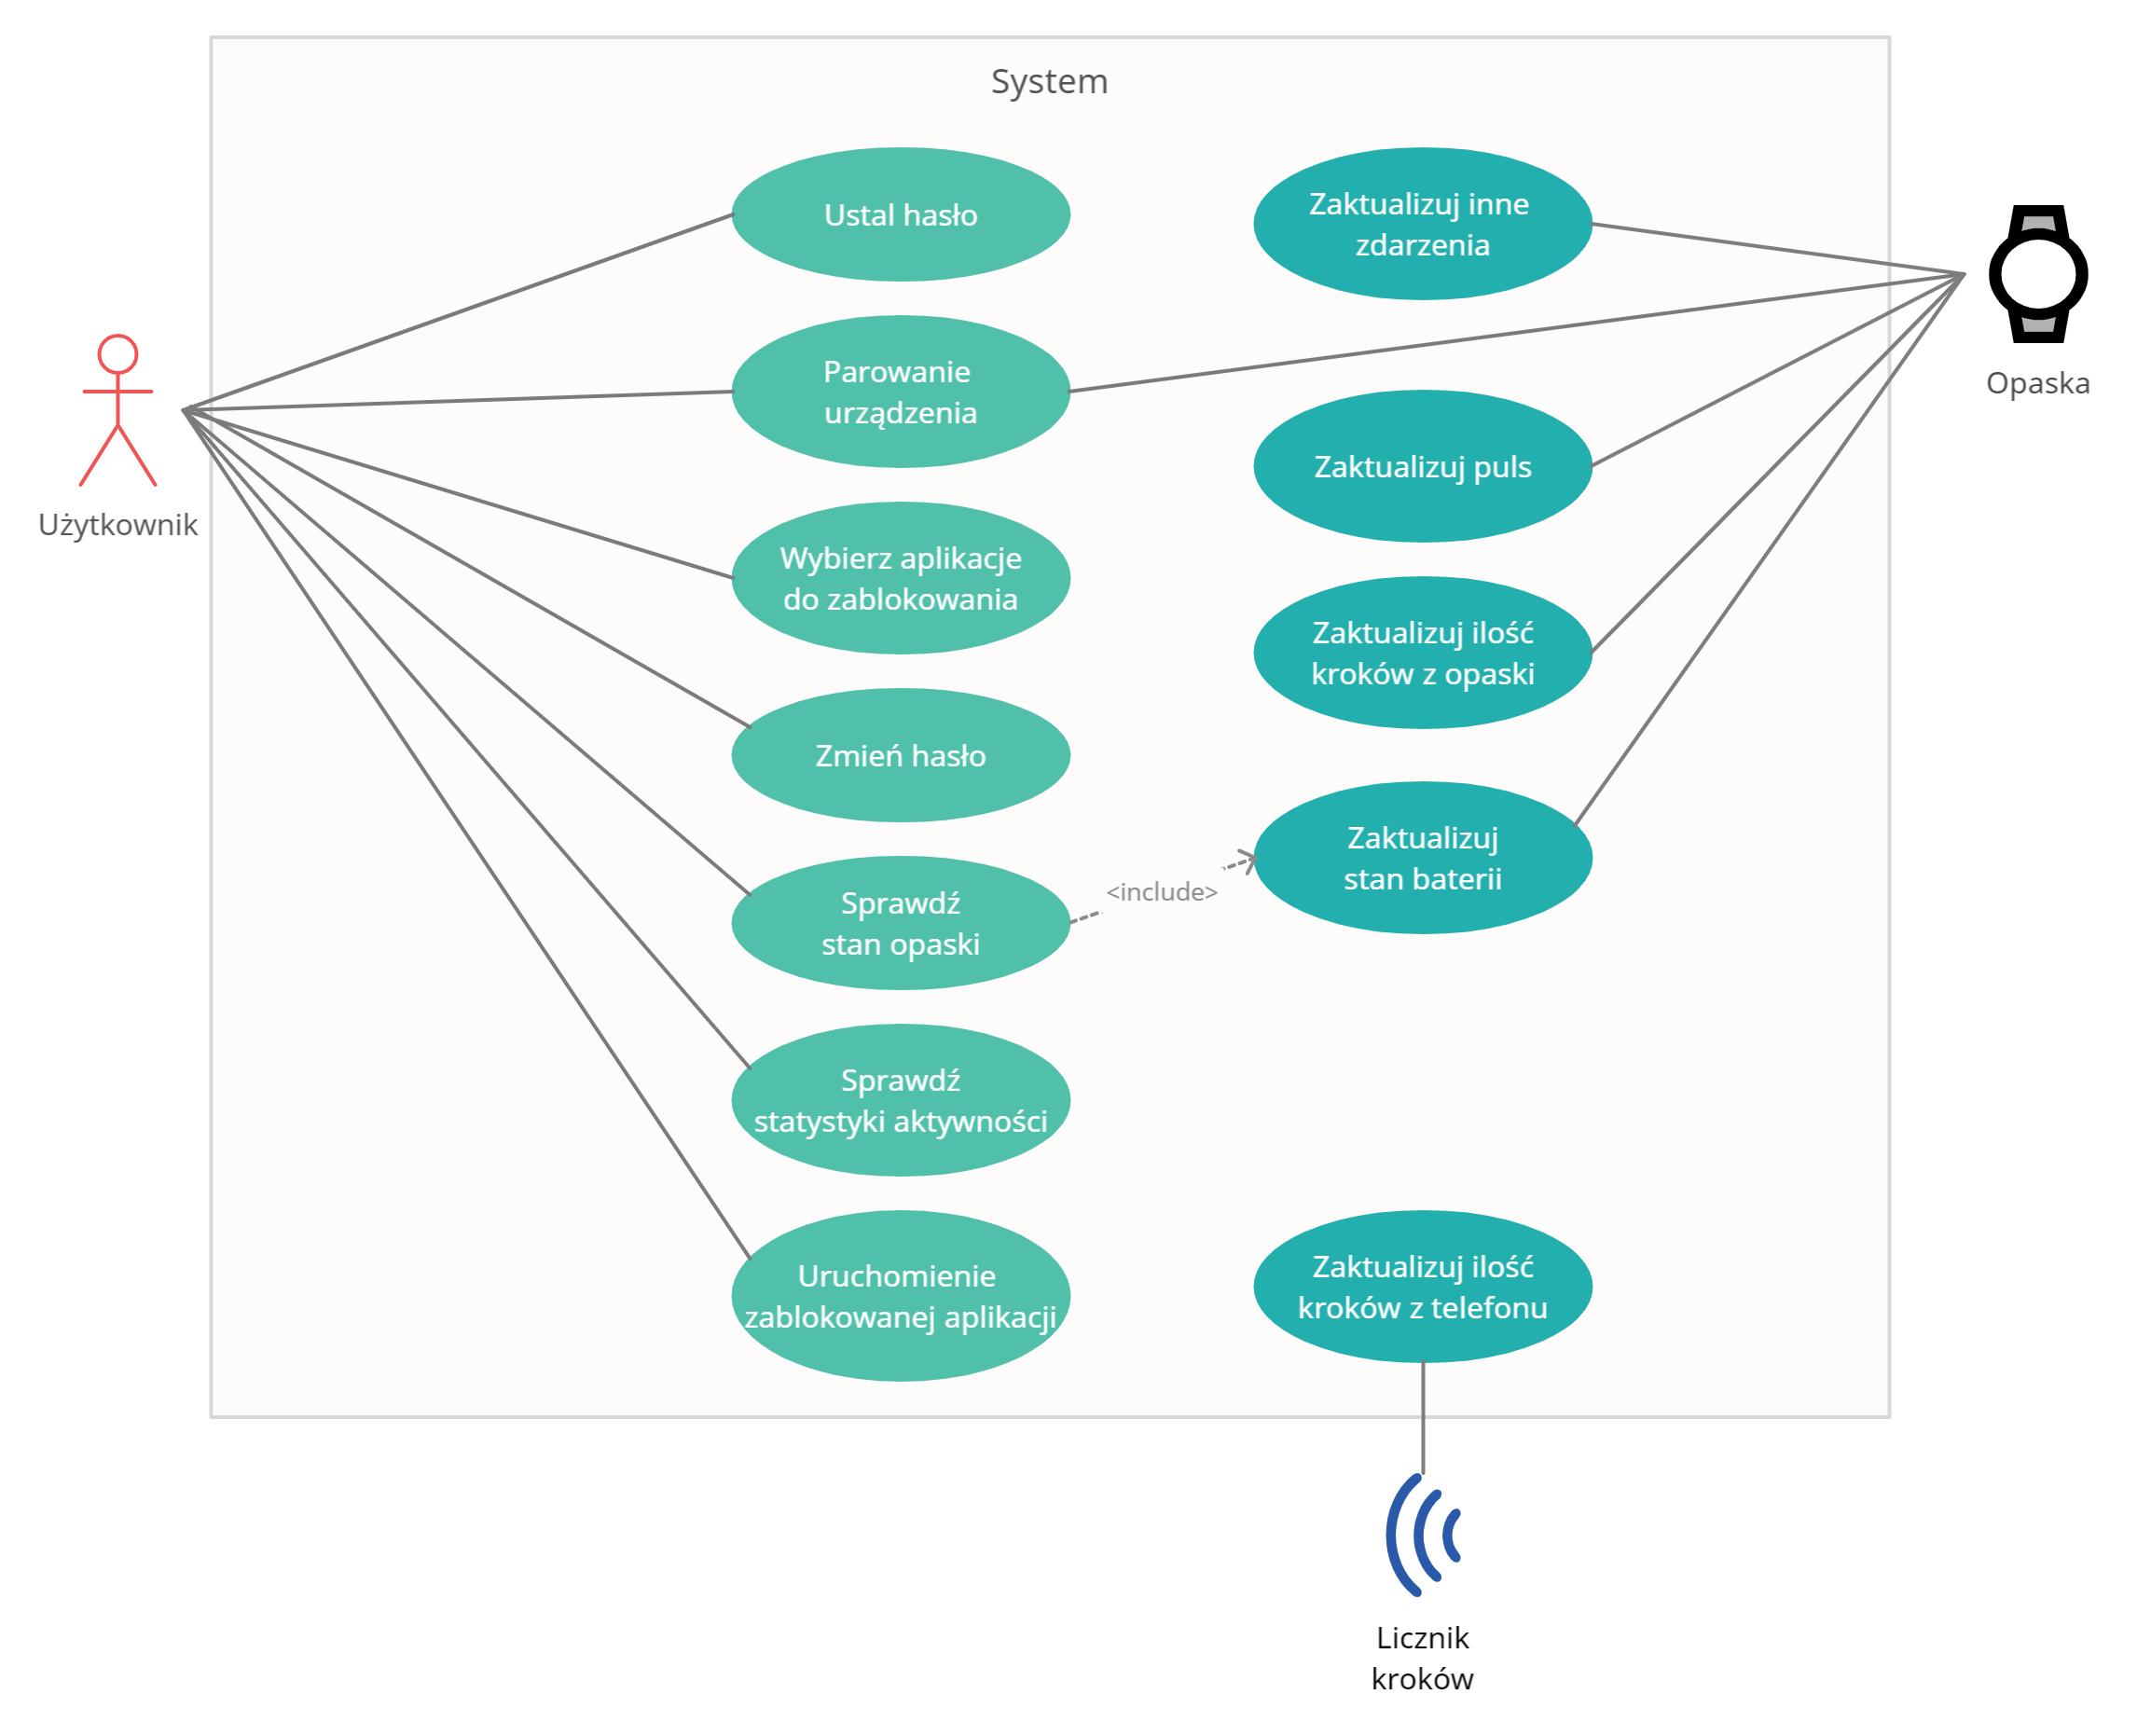
\includegraphics[width=0.9\textwidth]{UseCaseDiagram.png}
    \end{center}
    \caption{{\color{dgray}Diagram przypadków użycia w systemie.}} \label{use_case}
\end{figure}

\subsection{Ustal hasło}
W tym przypadku użytkownik aplikacji ustala hasło, które jest potrzebne przy odblokowywaniu dostępu do zablokowanych aplikacji. Aktorami są Użytkownik oraz System. Obecny przypadek użycia jest inicjowany przy pierwszym uruchomieniu aplikacji, kiedy nie istnieje jeszcze zaszyfrowany plik, w którym będzie przechowywane hasło. Po wykonaniu przypadku w systemie zostaje zarejestrowane hasło użytkownika, które będzie później wykorzystane w celu dezaktywacji blokady aplikacji. Scenariusz składa się z następującego przepływu głównego:
\begin{enumerate}
    \item Aplikacja wyświetla formularz zawierający pola Hasło oraz Powtórz hasło.
    \item Użytkownik wprowadza identyczne hasła do podanych pól oraz zatwierdza wprowadzone dane przyciskiem znajdującym się poniżej.
    \item System sprawdza zgodność haseł oraz czy spełniają wymagane kryteria.
    \item System tworzy zaszyfrowany plik i zapisuje w nim hasz hasła.
\end{enumerate}
Alternatywnie:
\newline\newline
\indent 3. Jeśli wprowadzone hasła nie są zgodne:
\begin{enumerate}[leftmargin=3\parindent]
    \item Zostaje wyświetlony komunikat o błędzie.
    \item Następuje powrót do kroku numer 2 w głównym przepływie.
\end{enumerate}

\subsection{Parowanie urządzenia}
W tym przypadku użytkownik aplikacji skanuje otoczenie, korzystając z modułu Bluetooth w poszukiwaniu najbliższej opaski MiBand, a następnie nawiązuje z nią pierwsze połączenie. Aktorami są Użytkownik, System oraz Opaska. Przypadek ten występuje przy pierwszym uruchomieniu systemu, kiedy zostało już ustalone hasło odblokowujące. Po zakończeniu system jest sparowany z opaską MiBand, z którą komunikacja jest kluczowym punktem działania systemu. W systemie zostaje także zapisany adres MAC opaski, dzięki czemu będzie można z łatwością ponownie połączyć się z nią. Główny przepływ składa się z następujących kroków:
\begin{enumerate}
    \item Użytkownik naciska przycisk ``Skan''.
    \item System rozpoczyna skanowanie urządzeń Bluetooth Low Energy w celu znalezienia Opaski.
    \item System wyświetla znalezione Opaski w formie listy. 
    \item Użytkownik wybiera Opaskę, do której się podłączy poprzez naciśnięcie na jej nazwę.
    \item System tworzy więź z wybraną Opaską i inicjuje pierwsze połączenie.
\end{enumerate}
Alternatywnie:
\newline\newline
\indent 3. Jeśli nie znaleziono żadnej Opaski:
\begin{enumerate}[leftmargin=3\parindent]
    \item Zostaje wyświetlony komunikat o błędzie.
    \item Następuje powrót do kroku numer 1 w głównym przepływie.
\end{enumerate}
\quad\newline
\indent 5. Jeśli wystąpi błąd połączenia z Opaską:
\begin{enumerate}[leftmargin=3\parindent]
    \item Następuje powrót do kroku numer 4 w głównym przepływie.
\end{enumerate}

\subsection{Wybierz aplikacje do zablokowania}
W tym przypadku użytkownik aplikacji wybiera z listy zainstalowanych aplikacji te, które będą blokowane przez system kiedy zostanie uruchomiona blokada. Aktorami są Użytkownik oraz System. Przypadek ten występuje, gdy istnieje plik z hasłem, opaska została sparowana, nie ma uruchomionej blokady oraz Użytkownik uruchomił aplikację. Po zakończeniu System posiada informację, na których aplikacjach uruchamiać blokadę. Główny przepływ składa się z następujących kroków:
\begin{enumerate}
    \item Użytkownik z poziomu głównego ekranu aplikacji przechodzi do Ustawień.
    \item Użytkownik wybiera opcję Zablokowane aplikacje.
    \item Użytkownik zaznacza aplikację z listy, którą chce zablokować bądź odblokować.
    \item System zapisuje aktualny stan aplikacji.
\end{enumerate}

\subsection{Zmień hasło}
W tym przypadku użytkownik aplikacji zmienia hasło odblokowujące dostęp do zablokowanych aplikacji. Aktorami są Użytkownik oraz System. Przypadek ten występuje, gdy istnieje plik z hasłem, opaska została sparowana, nie ma uruchomionej blokady oraz Użytkownik uruchomił aplikację. Po zakończeniu System posiada informację o nowym haśle, które będzie wykorzystywane od tej pory do odblokowywania dostępu. Główny przepływ składa się z następujących kroków:
\begin{enumerate}
    \item Użytkownik z poziomu głównego ekranu aplikacji wybiera opcję Ustawienia w dolnej nawigacji.
    \item Użytkownik wybiera opcję Zmień hasło.
    \item Użytkownik wpisuje odpowiednie wartości do pól Stare hasło, Nowe hasło oraz Powtórz nowe hasło oraz zatwierdza wprowadzone dane.
    \item System zapisuje hasz nowego hasła w zaszyfrowanym pliku.
\end{enumerate}
Alternatywnie: 
\newline\newline
\indent 3. Jeśli stare hasło jest błędne lub nowe hasło nie zgadza się z powtórzonym:
\begin{enumerate}[leftmargin=3\parindent]
    \item System wyświetla komunikat o błędnych wprowadzonych danych.
    \item Następuje powrót do kroku numer 3 w głównym przepływie.
\end{enumerate}
\quad\newline
\indent 4. Jeśli wystąpi błąd zapisu:
\begin{enumerate}[leftmargin=3\parindent]
    \item System wyświetla komunikat o błędzie zapisu.
    \item Następuje powrót do kroku numer 3 w głównym przepływie.
\end{enumerate}

\subsection{Sprawdź stan opaski}
W tym przypadku użytkownik aplikacji sprawdza podstawowe informacje na temat opaski oraz jej stan baterii. Aktorami są Użytkownik, System oraz Opaska. Przypadek ten występuje, gdy istnieje plik z hasłem, opaska została sparowana, nie ma uruchomionej blokady oraz Użytkownik uruchomił aplikację. Po zakończeniu Użytkownik zna stan baterii oraz inne informacje o Opasce, a System zyskuje odświeżony stan baterii Opaski. Głowny przepływ składa się z następujących kroków:
\begin{enumerate}
    \item Użytkownik z poziomu głównego ekranu aplikacji wybiera opcję Opaska w dolnej nawigacji.
    \item System wyświetla zapisane wcześniej informacje o Opasce.
    \item Przejdź do przypadku Zaktualizuj stan baterii
    \item System aktualizuje wartość baterii na ekranie.
\end{enumerate}
Alternatywnie:
\newline\newline
\indent 2. Jeśli nie zapisano wcześniej informacji o Opasce:
\begin{enumerate}[leftmargin=3\parindent]
    \item System wyświetla w brakujących polach wartość Nieznane.
    \item Następuje przejście do kroku numer 3 w głównym przepływie.
\end{enumerate}
\quad\newline
\indent 3. Jeśli nastąpi nagła utrata połączenia z Opaską:
\begin{enumerate}[leftmargin=3\parindent]
    \item Pomiń następny krok w głównym przepływie.
\end{enumerate}

\subsection{Sprawdź statystyki aktywności}
W tym przypadku użytkownik aplikacji sprawdza proste statystyki zarejestrowanej dziennej aktywności. Aktorami są Użytkownik oraz System. Przypadek ten występuje, gdy istnieje plik z hasłem, opaska została sparowana, nie ma uruchomionej blokady oraz Użytkownik uruchomił aplikację. Po zakończeniu Użytkownik zna ilość zarejestrowanych kroków oraz ostatnią zarejestrowaną wartość pulsu. Główny przepływ składa się z następujących kroków:
\begin{enumerate}
    \item Użytkownik z poziomu głównego ekranu aplikacji wybiera opcję Statystyki w dolnej nawigacji.
    \item System wyświetla ostatnie zapisane wartości dziennych kroków oraz pulsu.
    \item System aktualizuje wyświetlane wartości, gdy zostaną zapisane nowe.
\end{enumerate}

\subsection{Uruchomienie zablokowanej aplikacji}
W tym przypadku użytkownik aplikacji próbuje uruchomić aplikację z listy zablokowanych podczas, gdy uruchomiona jest blokada. Aktorami są Użytkownik i System. Przypadek ten występuje, gdy istnieje plik z hasłem, opaska została sparowana oraz aplikacja pracuje w trybie blokady. Po zakończeniu Użytkownik posiada autoryzację do interakcji z blokowanymi aplikacjami, a System przechodzi w tryb monitorowania. Główny przepływ składa się z następujących kroków:
\begin{enumerate}
    \item Użytkownik uruchamia aplikację z listy zablokowanych.
    \item System przenosi Użytkownika w ekran wprowadzania hasła.
    \item Użytkownik wprowadza hasło i zatwierdza.
    \item System wyłącza blokadę i uruchamia usługę monitorującą.
\end{enumerate}
Alternatywnie:
\newline\newline
\indent 3. Jeśli Użytkownik wprowadził błędne hasło:
\begin{enumerate}[leftmargin=3\parindent]
    \item System wyświetla komunikat o błędnym haśle.
    \item Następuje ponowne wykonanie kroku 3 z głównego przepływu.
\end{enumerate}

\subsection{Zaktualizuj inne zdarzenia}

\subsection{Zaktualizuj puls}

\subsection{Zaktualizuj ilość kroków z opaski}

\subsection{Zaktualizuj stan baterii}

\subsection{Zaktualizuj ilość kroków z telefonu}

\section{Diagram komponentów}

W tej sekcji należy przedstawić diagramy komponentów dla odpowiednich elementów systemu zidentyfikowane na podstawie wcześniejszych rozważań

\section{Diagramy stanów}

W tej sekcji należy przedstawić diagramy stanów w których może znaleźć się system. Diagramy te są szczególnie istotne przy projektowaniu systemów czasu rzeczywistego.

\section{Projekt bazy danych}

W tej sekcji należy przedstawić projekt bazy danych. Należy omówić wycinek rzeczywistości i odpowiadające mu zidentyfikowane elementy systemu, których wartości będą podlegać utrwalaniu. Należy przedyskutować wybór typów danych dla atrybutów poszczególnych obiektów.  

\section{Opis protokołów}
\begin{itemize}
    \item inicjalizacja komunikacji z opaską
\end{itemize}

W projektowanym systemie główną rolę gra inteligentna opaska. Komunikuje się ona ze smartfonem przy użyciu technologii Bluetooth Low Energy oraz protokołu ATT. BLE w porównaniu
do klasycznego połączenia Bluetooth wykorzystuje znacznie niższe zasoby energii zachowując podobny zasięg, dzięki czemu znalazło
szerokie zastosowanie w urządzeniach peryferyjnych.
\subsection{Protokół ATT}
Protokół Attribute pozwala urządzeniom odczytywać i zapisywać drobne dane przechowywane na serwerze.
Przechowywane wartości są nazywane atrybutami. Atrybuty identyfikowane są poprzez
UUID, aby określić typ przechowywanych w nich danych. UUID mogą być powszechnie znanymi
numerami zdefiniowanymi w oficjalnej specyfikacji Bluetooth albo być
określone przez producenta jako 128-bitowa liczba. Wiadomości w tym
protokole są przesyłane przez kanały L2CAP, znanymi jako nośniki ATT. W ATT
występują dwie role: Klienta oraz Serwera. Urządzenie może pełnić obie te role
jednocześnie. Serwer przechowuje atrybuty oraz akceptuje żądania, komendy
oraz potwierdzenia pochodzące od klienta. Serwer wysyła także odpowiedzi na
żądania, a gdy zostanie skonfigurowany przez wyższą warstwę, wysyła asynchronicznie powiadomienia
do klienta, kiedy występują na nim określone zdarzenia.
\subsection{GATT}
Komunikacja aplikacji z opaską odbywa się przy wykorzystaniu GATT (Generic Attribute Profile). Jest to technologia zbudowana na protokole Attribute (ATT), która
ustala przebieg powszechnych operacji oraz framework dla danych transportowanych przez ATT.
GATT określa format danych przesyłanych przez protokół Attribute. Atrybuty są
formatowane jako Usługi oraz Charakterystyki. Usługi są zbiorem danych oraz
przypisanych im zachowań niezbędnych do zapewnienia określonej funkcji urządzenia.
Z kolei Charakterystyki są wartościami użytymi w Usłudze wraz z ich właściwościami
oraz informacjami o tym jak są wyświetlane bądź reprezentowane. Dzięki
wykorzystaniu określonej struktury danych przez GATT możliwe jest przeglądanie
dostępnych Usług oraz Charakterystyk, nawet gdy klient nie jest wyspecjalizowany
pod dany serwer.
\subsection{Komunikacja z MiBand 3}
